% !TeX root = ../main.tex

\chapter{系统设计与实现}

本文第三四章中详细介绍了...,
这为最终系统和我财富自由的实现提供了技术基础。...

本章将负责介绍系统的设计与实现,同时这也是本文的最终目的。


\section{设计架构}



pnpm 管理依赖的性能相较 npm、yarn 提升显著,如图~\ref{fig:pnpm-npm-yarn-benchmark}。
\definecolor{pnpm}{HTML}{f1b03d}
\definecolor{npm}{HTML}{be4439}
\definecolor{yarn}{HTML}{458db9}
\definecolor{yarnPnp}{HTML}{5ca9f8}
\begin{figure}
  \centering
  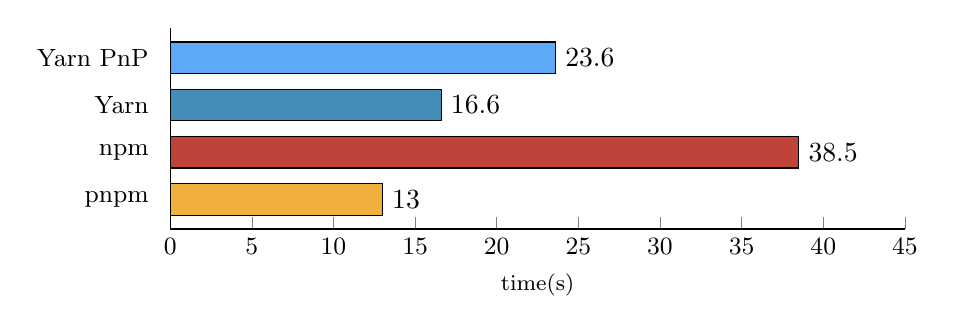
\begin{tikzpicture}
    \begin{axis}[
        xbar=0pt,
        /pgf/bar shift=0pt,
        legend style={
        legend columns=4,
            at={(xticklabel cs:0.5)},
            anchor=north,
            draw=none
        },
        % ytick={pnpm,npm,Yarn,{Yarn PnP}},
        ytick={0,...,4},
        ytick style={draw=none},% <- added
        axis y line*=none,
        axis x line*=bottom,
        legend style={font=\footnotesize},
        label style={font=\footnotesize},
        width=.9\textwidth,
        bar width=4mm,
        yticklabels={
            {pnpm}, 
            {npm}, 
            {Yarn}, 
            {Yarn PnP},
        },
        xlabel={time(s)},
        xmin=0,
        xmax=45,
        area legend,
        y=6mm,
        enlarge y limits={abs=0.625},
        nodes near coords,
        nodes near coords style={text=black},
        every axis plot/.append style={fill},
        tick label style={font=\small},
    ]
      \addplot[fill=pnpm] coordinates {(13,0)};
      \addplot[fill=npm] coordinates {(38.5,1)};
      \addplot[xbar, fill=yarn] coordinates {(16.6,2)};
      \addplot[xbar, fill=yarnPnp] coordinates {(23.6,3)};
    \end{axis}  
  \end{tikzpicture}
  \caption{Monorepo 中 Yarn/pnpm/npm Benchmark}
  \label{fig:pnpm-npm-yarn-benchmark}
\end{figure}

TIKZ 也可以画思维导图,如图~\ref{fig:advjs-modules}。

\begin{figure}[htb]
  \centering
  \begin{tikzpicture}[
    scale=1,
    mindmap, grow cyclic, every node/.style=concept, concept color=purple!20, 
    level 1/.append style={level distance=5cm,sibling angle=90},
    level 2/.append style={level distance=3cm,sibling angle=45},]
    
    \node{ADV.JS}
    child[concept color=green!20] { node {Ecosystem}
      child { node {create-adv 脚手架}}
      child { node {Template 模版示例}}
      child { node {UI 主题}}
    }
    child[concept color=yellow!20] { node {Parser 剧本解析器}
      child { node {AdvScript 语法解析}}
      child { node {unplugin-adv 解析插件}}
      child { node {Vitest 测试}}
      child { node {TypeScript 节点类型定义}}
    }
    child[concept color=blue!20] { node {Editor 编辑器}
      child { node {VRM 编辑器}}
      child { node {剧本编辑器}}
      child { node {VSCode 语法高亮}}
    }
    child[concept color=teal!20] { node {Client 客户端}
      child { node {Adv Ui Components}}
      child { node {Core 核心逻辑}}
      child { node {Store 状态管理}}
      child { node {theme-default}}
    }
    ;
  \end{tikzpicture}
  \caption{模块关系图}
  \label{fig:advjs-modules}
\end{figure}

流程图可以看这里。

\url{https://www.overleaf.com/learn/latex/LaTeX_Graphics_using_TikZ%3A_A_Tutorial_for_Beginners_(Part_3)%E2%80%94Creating_Flowcharts}


\section{客户端开发}

...


\section{系统实现}

各几节介绍一下系统实现的关键技术吧



\section{系统展示}

可以贴点图什么的……

\begin{figure}[htbp]
  \centering
  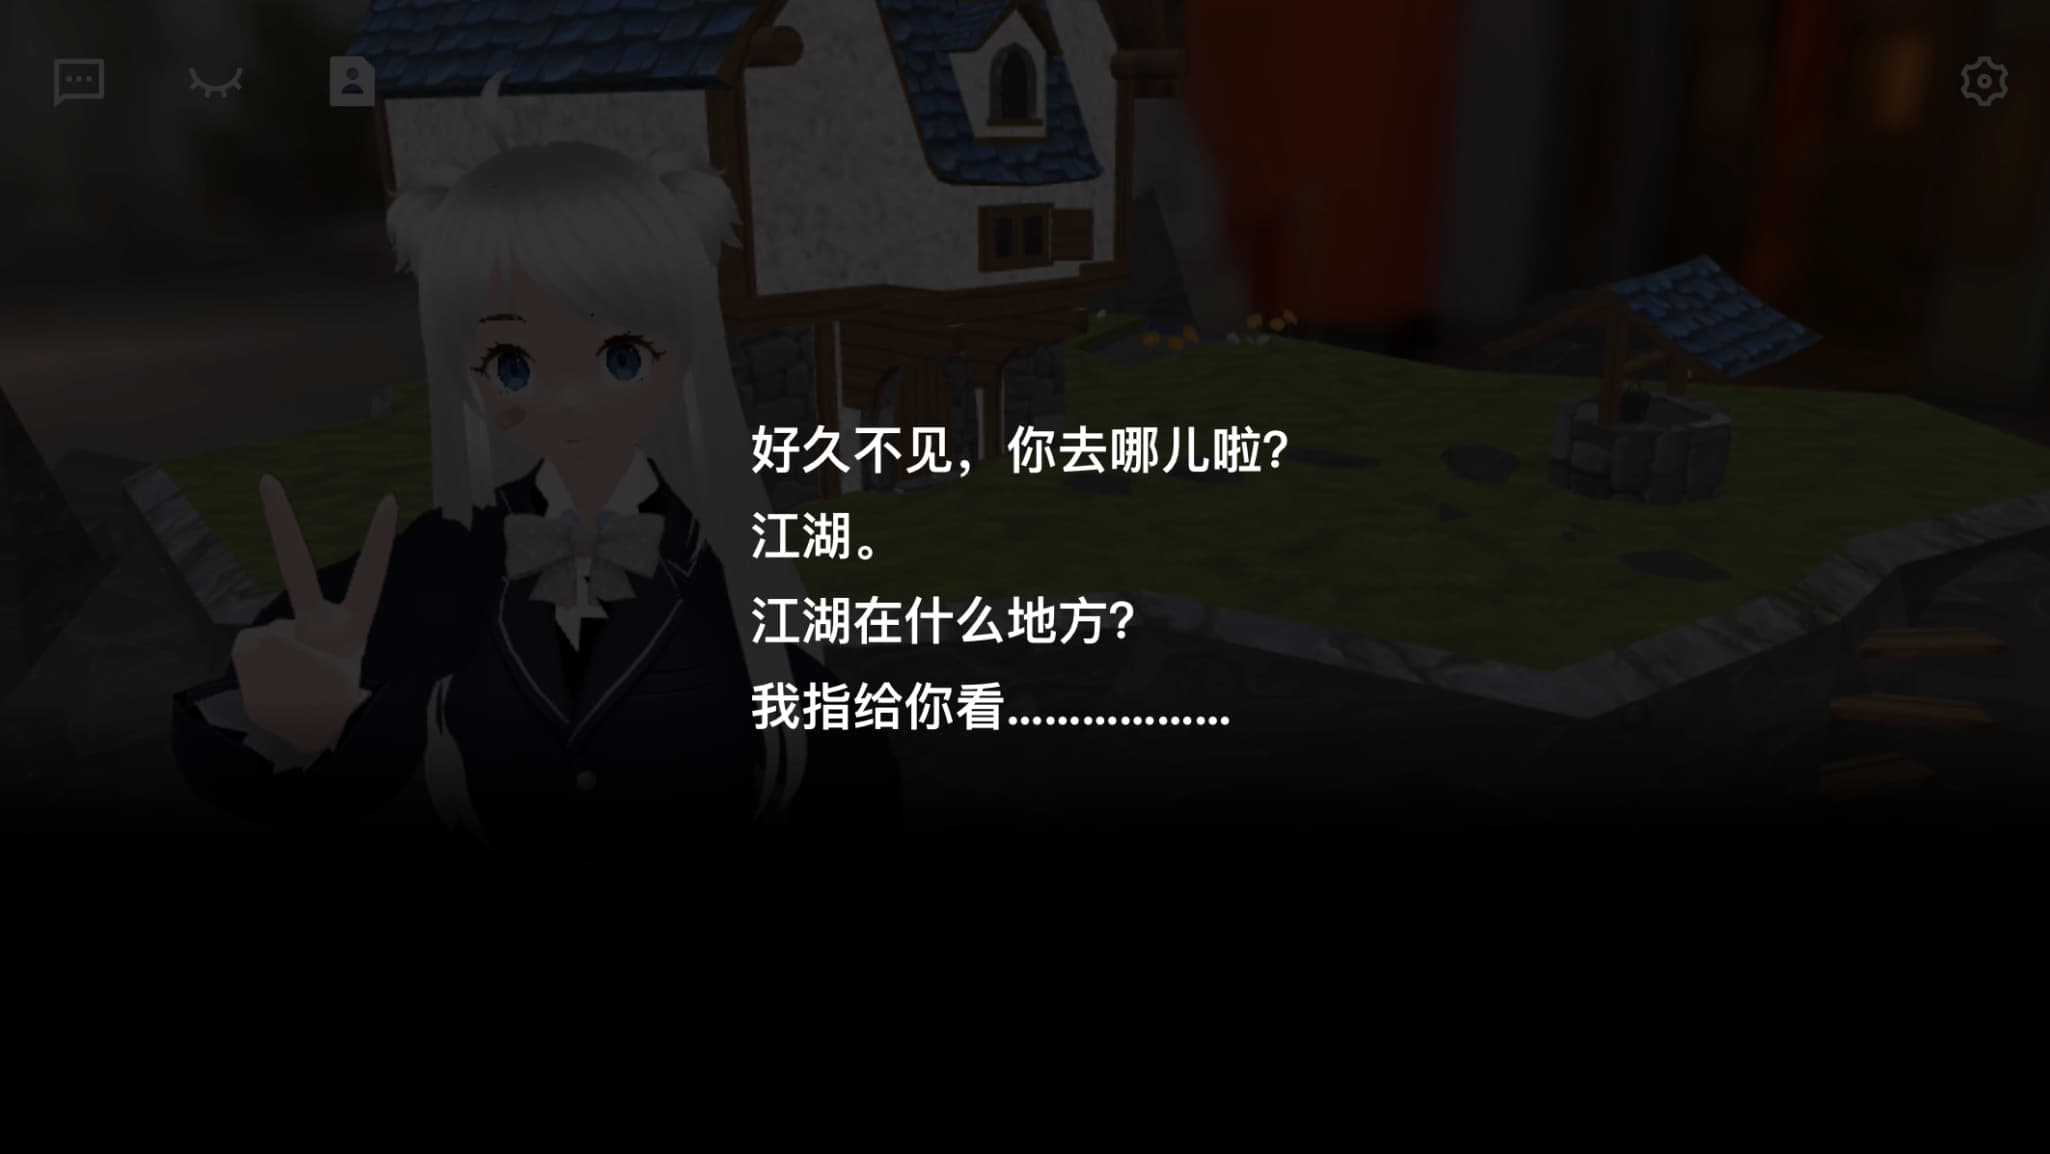
\includegraphics[width=.5\linewidth]{advjs-black.jpg}
  \caption{测试}
  \label{fig:advjs-debug}
\end{figure}


\section{系统测试与评价}

测试、调查

\section{本章小结}

本章...
